% Source printed pp. 50-54.
\section{Grassmann 概形的射影性}\label{src:2.2}
\begin{epigraph}
做数学的艺术, 在于找到那个蕴含所有一般性萌芽的特殊情形.
\epigraphauthor{David Hilbert}
\end{epigraph}
Grassmann 概形为利用函子方法构造射影模空间提供了热身, 也在 Hilb 与 Quot 的可表性和射影性论证中起着重要作用.
\subsection{可由概形表出}\label{src:2.2.1-subsection}
我们将给出 $\Gr(q,n)=\Gr(q,\mathcal O_{\operatorname{Spec}\mathbb Z}^{\oplus n})$ 的一个由可表子函子组成的 Zariski 开覆盖, 证明它可由概形表出(命题~\bookref{2.2.5}); 见定义~\bookref{1.3.42}.
给定大小为 $q$ 的子集 $I\subseteq\{1,\ldots,n\}$, 定义子函子 $\Gr_I\subseteq\Gr(q,n)$: 
\begin{equation}\label{src:2.2.1}
\begin{aligned}
\Gr_I:\Sch&\longrightarrow\Sets,\\
T&\longmapsto
\left\{\begin{array}{l}
\text{商 $[p:\mathcal O_T^{\oplus n}\twoheadrightarrow Q]\in\Gr(q,n)(T)$, }\\
\text{使复合 $\mathcal O_T^{\oplus I}\xrightarrow{e_I}
\mathcal O_T^{\oplus n}\xrightarrow{p}Q$ 为同构}
\end{array}\right\},
\end{aligned}
\end{equation}
其中 $e_I$ 为典范包含映射.
\begin{lemma}\label{src:2.2.2}
对每个大小为 $q$ 的子集 $I\subseteq\{1,\ldots,n\}$, 函子 $\Gr_I$ 可由仿射空间 $\mathbb A_{\mathbb Z}^{q\times(n-q)}$ 表出.
\end{lemma}
\begin{proof}
可以假设 $I=\{1,\ldots,q\}$. 定义函子映射 $\phi:\mathbb A^{q\times(n-q)}\to\Gr_I$: 在概形 $T$ 上, 将由 $T$ 上整体函数组成的 $q\times(n-q)$ 矩阵 $f=(f_{i,j})_{1\leq i\leq q,\ 1\leq j\leq n-q}$ 映至商
\begin{equation}\label{src:2.2.3}
\left(\begin{array}{cccc|ccc}
1&&&&f_{1,1}&\cdots&f_{1,n-q}\\
&1&&&f_{2,1}&\cdots&f_{2,n-q}\\
&&\ddots&&\vdots&&\vdots\\
&&&1&f_{q,1}&\cdots&f_{q,n-q}
\end{array}\right):
\mathcal O_T^{\oplus n}\longrightarrow\mathcal O_T^{\oplus q}.
\end{equation}
$\phi(T):\mathbb A^{q\times(n-q)}(T)\to\Gr_I(T)$ 的单射性来自如下事实: 任意两个写成~\eqref{src:2.2.3}~形式且在 $\Gr_I$ 中等价的商, 必由同样的方程定义.
为说明满射性, 取 $[p:\mathcal O_T^{\oplus n}\twoheadrightarrow Q]\in\Gr_I(T)$, 按定义, $\mathcal O_T^{\oplus I}\xrightarrow{e_I}\mathcal O_T^{\oplus n}\xrightarrow{p}Q$ 为同构.
重言交换图
\[
\begin{tikzcd}
\mathcal O_T^{\oplus n}\arrow[r,"p"]\arrow[dr,"(p\circ e_I)^{-1}\circ p"']&
Q\arrow[d,"(p\circ e_I)^{-1}"]\\
&\mathcal O_T^{\oplus I}
\end{tikzcd}
\]
表明
\[
[p:\mathcal O_T^{\oplus n}\twoheadrightarrow Q]
=[(p\circ e_I)^{-1}\circ p:\mathcal O_T^{\oplus n}\twoheadrightarrow
\mathcal O_T^{\oplus I}]\in\Gr(q,n)(T).
\]
由于复合
$\mathcal O_T^{\oplus I}\xrightarrow{e_I}\mathcal O_T^{\oplus n}
\xrightarrow{(p\circ e_I)^{-1}}\mathcal O_T^{\oplus I}$
为恒等映射, 对应于 $(p\circ e_I)^{-1}\circ p$ 的 $q\times n$ 矩阵必为~\eqref{src:2.2.3}~的形式, 其中 $f_{i,j}\in\Gamma(T,\mathcal O_T)$.
因此, $\phi(T)(\{f_{i,j}\})=[p:\mathcal O_T^{\oplus n}\twoheadrightarrow Q]\in\Gr(q,n)(T)$.
\end{proof}
\begin{lemma}\label{src:2.2.4}
当 $I$ 遍历所有大小为 $q$ 的子集时, 子函子族 $\{\Gr_I\}$ 为 $\Gr(q,n)$ 的一个 Zariski 开覆盖.
\end{lemma}
\begin{proof}
对固定的子集 $I$, 先证明 $\Gr_I\subseteq\Gr(q,n)$ 为开子函子.
为此, 考虑概形 $T$ 和对应于商 $p:\mathcal O_T^{\oplus n}\to Q$ 的态射 $T\to\Gr(q,n)$.
记复合 $p\circ e_I:\mathcal O_T^{\oplus I}\to Q$ 的余核为 $C$.
注意, 若 $C=0$, 则 $p\circ e_I$ 为同构.
函子的纤维积
\[
\begin{tikzcd}[column sep=large]
T_I\arrow[r]\arrow[d]\arrow[dr,phantom,"\square"]&
T\arrow[d,"{[\mathcal O_T^{\oplus n}\xrightarrow{p}Q]}"]\\
\Gr_I\arrow[r]&\Gr(q,n)
\end{tikzcd}
\]
可由开子概形 $U=T\setminus\operatorname{Supp}(C)$ 表出(鼓励读者验证这一断言).
注意, 即使 $T$ 不是 Noether 概形, $\operatorname{Supp}(C)\subseteq T$ 仍为闭集, 因为 $C$ 为有限型拟凝聚层.

为检验 $\coprod_IT_I\to T$ 的满射性, 取点 $t\in T$.
由于 $p\otimes\kappa(t):\kappa(t)^n\twoheadrightarrow Q\otimes\kappa(t)$ 为向量空间的满射, $q\times n$ 矩阵 $p\otimes\kappa(t)$ 有一个由子集 $I$ 确定的非零 $q\times q$ 子式.
这意味着 $[p\otimes\kappa(t)]\in T_I(\kappa(t))$.
\end{proof}
引理~\bookref{2.2.2}~和~\bookref{2.2.4}~共同推出: 
\begin{proposition}\label{src:2.2.5}
函子 $\Gr(q,n)$ 可由概形表出.
\end{proposition}
\begin{exercise}[简单]\label{src:2.2.6}
证明 $\Gr(q,n)$ 是 $\mathbb Z$ 上相对维数为 $q(n-q)$ 的光滑概形.
\end{exercise}
\begin{exercise}[适合练习]\label{src:2.2.7}
利用固有性的赋值判别法证明 $\Gr(q,n)\to\operatorname{Spec}\mathbb Z$ 固有.
\end{exercise}
\subsection{Grassmann 概形的射影性}\label{src:2.2.2-subsection}
我们将显式给出一个射影嵌入, 证明 Grassmann 概形 $\Gr(q,n)$ 射影.
\newterm{Plücker 嵌入}{Plücker embedding}是函子映射
\[
\begin{aligned}
P:\Gr(q,n)&\longrightarrow
\mathbb P\left(\bigwedge^q\mathcal O_{\operatorname{Spec}\mathbb Z}^{\oplus n}\right),\\
[\mathcal O_T^{\oplus n}\twoheadrightarrow Q]&\longmapsto
\left[\bigwedge^q\mathcal O_T^{\oplus n}\longrightarrow\bigwedge^qQ\right],
\end{aligned}
\]
上式定义在概形 $T$ 上. 由于两边均可由概形表出, 由 Yoneda 引理(\bookref{1.3.12}), 态射 $P$ 对应于一个概形态射.
\begin{proposition}\label{src:2.2.8}
态射 $P:\Gr(q,n)\to\mathbb P(\bigwedge^q\mathcal O_{\operatorname{Spec}\mathbb Z}^{\oplus n})$ 为闭浸入.
特别地, $\Gr(q,n)$ 是 $\mathbb Z$ 上的射影概形.
\end{proposition}
\begin{proof}
大小为 $q$ 的子集 $I\subseteq\{1,\ldots,n\}$ 对应于 $\mathbb P(\bigwedge^q\mathcal O_{\operatorname{Spec}\mathbb Z}^{\oplus n})$ 上的坐标 $x_I$.
记 $x_I\neq0$ 的开轨迹为 $\mathbb P(\bigwedge^q\mathcal O_{\operatorname{Spec}\mathbb Z}^{\oplus n})_I$.
注意, 它是参数化线丛商 $\bigwedge^q\mathcal O_S^{\oplus n}\to L$ 的子函子, 其中复合 $\mathcal O_S\xrightarrow{e_I}\bigwedge^q\mathcal O_S^{\oplus n}\to L$ 为同构(第一个映射为第 $I$ 项的包含映射).
因此, 有函子的 Cartesian 图
\[
\begin{tikzcd}[column sep=large]
\Gr_I\arrow[r,"P_I"]\arrow[d]\arrow[dr,phantom,"\square"]&
\mathbb P(\bigwedge^q\mathcal O_{\operatorname{Spec}\mathbb Z}^{\oplus n})_I\arrow[d]\\
\Gr(q,n)\arrow[r,"P"]&
\mathbb P(\bigwedge^q\mathcal O_{\operatorname{Spec}\mathbb Z}^{\oplus n}),
\end{tikzcd}
\]
其中 $\Gr_I$ 定义于~\eqref{src:2.2.1}.
由于这些射影空间的开子概形构成 Zariski 开覆盖, 只需证明每个映射
\[
P_I:\Gr(q,n)_I\longrightarrow
\mathbb P(\bigwedge^q\mathcal O_{\operatorname{Spec}\mathbb Z}^{\oplus n})_I
\]
都是闭浸入.

为简便起见, 假设 $I=\{1,\ldots,q\}$.
在引理~\bookref{2.2.2}~的同构 $\Gr_I\cong\mathbb A_{\mathbb Z}^{q\times(n-q)}$ 及
$\mathbb P(\bigwedge^q\mathcal O_{\operatorname{Spec}\mathbb Z}^{\oplus n})_I
\cong\mathbb A_{\mathbb Z}^{\binom nq-1}$
之下, 态射 $P_I$ 对应于映射
\[
\mathbb A_{\mathbb Z}^{q\times(n-q)}
\longrightarrow\mathbb A_{\mathbb Z}^{\binom nq-1}.
\]
它将 $q\times(n-q)$ 矩阵 $\{x_{i,j}\}$ 映至右边的一个元素: 对不同于 $I$, 长度为 $q$ 的子集 $J\subset\{1,\ldots,n\}$, 其第 $J$ 坐标为如下 $q\times n$ 分块矩阵的 $\{1,\ldots,q\}\times J$ 子式: 
\[
\left(\begin{array}{cccc|ccc}
1&&&&x_{1,1}&\cdots&x_{1,n-q}\\
&1&&&x_{2,1}&\cdots&x_{2,n-q}\\
&&\ddots&&\vdots&&\vdots\\
&&&1&x_{q,1}&\cdots&x_{q,n-q}
\end{array}\right).
\]
$\mathbb A_{\mathbb Z}^{q\times(n-q)}$ 上的坐标 $x_{i,j}$ 是对应于子集
$\{1,\ldots,\widehat i,\ldots,q,q+j\}$ 的坐标的拉回(见图~\bookref{2.5.5}).
这表明对应的环映射满射, 因而 $P_I$ 为闭浸入.
\end{proof}
\begin{figure}[H]
\centering% Source printed p. 52, mathematical labels only, 400 DPI.
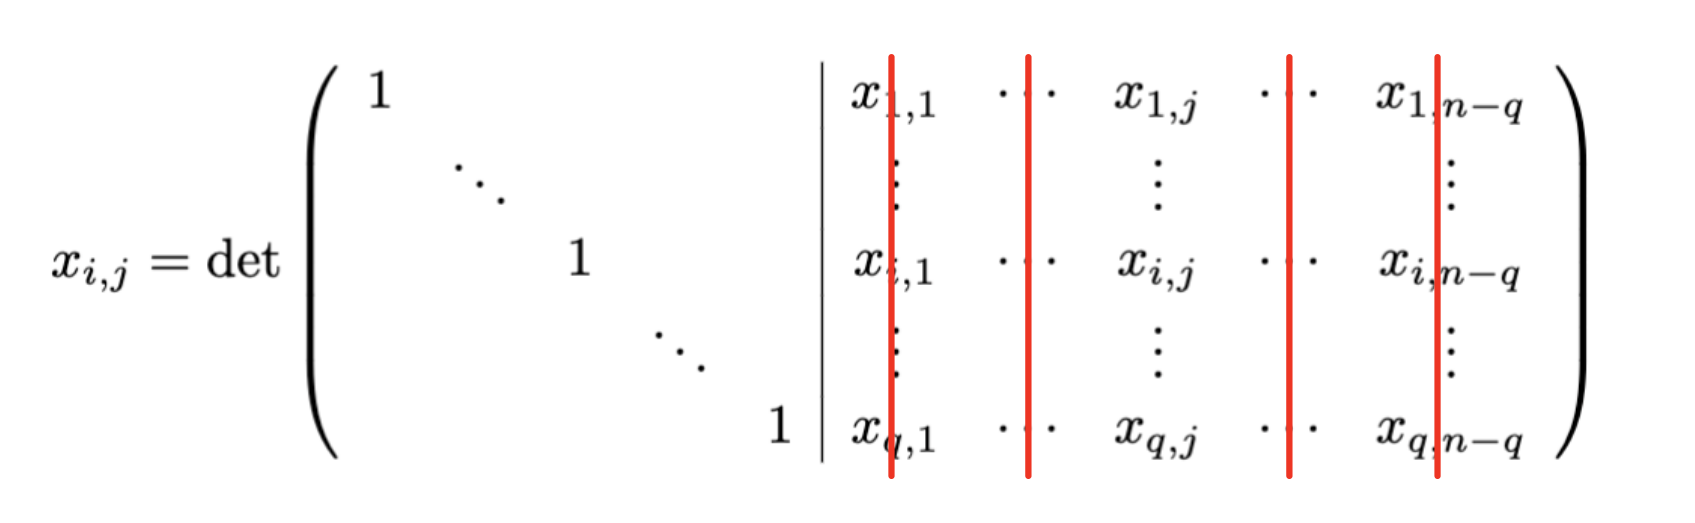
\includegraphics[width=.68\textwidth]{figures/fig-2.2.9.png}

\caption{去掉第 $i$ 列以及 $q+1,\ldots,n$ 中除 $q+j$ 外的所有列, 所得子式恰为 $x_{i,j}$.}\label{src:2.2.9}
\end{figure}
\[
x_{i,j}=\det
\left(\begin{array}{ccccc|ccccc}
1&&&&&x_{1,1}&\cdots&x_{1,j}&\cdots&x_{1,n-q}\\
&\ddots&&&&\vdots&&\vdots&&\vdots\\
&&1&&&x_{i,1}&\cdots&x_{i,j}&\cdots&x_{i,n-q}\\
&&&\ddots&&\vdots&&\vdots&&\vdots\\
&&&&1&x_{q,1}&\cdots&x_{q,j}&\cdots&x_{q,n-q}
\end{array}\right)
\]
\begin{exercise}[适合练习]\label{src:2.2.10}
对域 $k$, 定义 $\Gr(q,n)_k:=\Gr(q,n)\times_{\mathbb Z}k$, 取对应于商 $Q=k^n/K$ 的点 $p\in\Gr(q,n)_k$.
证明切空间与 $k$-线性映射 $K\to Q$ 的向量空间之间存在自然双射
\[
T_p(\Gr(q,n)_k)\xrightarrow{\sim}\operatorname{Hom}_k(K,Q).
\]
\end{exercise}
\begin{exercise}[适合练习]\label{src:2.2.11}
利用 $\Gr(q,n)$ 的固有性赋值判别法(习题~\bookref{2.2.7}), 给出射影性的另一证明.
\end{exercise}
\begin{exercise}[困难]\label{src:2.2.12}
证明 $\Gr(q,n)$ 可等同于商 $U/\operatorname{GL}_q$, 其中 $U\subseteq\mathbb A^{q\times n}$ 为满秩 $q\times n$ 矩阵组成的子集; 也可等同于商 $\operatorname{GL}_n/H$, 其中
\[
H=\left\{\left.
\begin{pmatrix}A&B\\0&C\end{pmatrix}
\ \right|\ A\in\operatorname{GL}_q,\ B\in\mathbb A^{q\times(n-q)},\
C\in\operatorname{GL}_{n-q}\right\}\subseteq\operatorname{GL}_n.
\]
\end{exercise}
\begin{exercise}[困难]\label{src:2.2.13}
证明 $\operatorname{Pic}(\Gr(q,n))\cong\mathbb Z$, 且由 Plücker 线丛生成.
\end{exercise}
\begin{exercise}[旗簇]\label{src:2.2.14}
固定正整数 $n$ 及严格递减的整数序列 $n>q_1>\cdots>q_s>0$.
证明将概形 $S$ 映至商序列
\[
\mathcal O_S^{\oplus n}\twoheadrightarrow V_1\twoheadrightarrow
\cdots\twoheadrightarrow V_s
\]
的同构类的函子 $\Sch\to\Sets$, 可由 $\mathbb Z$ 上的射影概形表出, 其中每个 $V_i$ 都是 $S$ 上秩为 $q_i$ 的向量丛.
\end{exercise}
\subsection{相对版本}\label{src:2.2.3-subsection}
我们证明: 对 Noether 概形 $S$ 上任意向量丛 $V$, 函子 $\Gr(q,V)$ 在 $S$ 上可表且射影.
\begin{proof}[定理~\bookref{2.1.1}~的证明]
若 $V$ 为 $S$ 上秩为 $n$ 的向量丛, 则有相对 Plücker 嵌入
\[
\begin{aligned}
P:\Gr(q,V)&\longrightarrow\mathbb P\left(\bigwedge^qV\right),\\
[V_T\twoheadrightarrow Q]&\longmapsto
\left[\bigwedge^qV_T\longrightarrow\bigwedge^qQ\right],
\end{aligned}
\]
上式定义在 $S$-概形 $T$ 上, 是 $S$ 上的函子态射.
由于 $\mathbb P(\bigwedge^qV)$ 在 $S$ 上射影, 只需证明这一态射可由闭浸入表出.
这一性质可在 Zariski 局部检验: 若 $U\subseteq S$ 为使 $V$ 平凡的开子概形, 则 $\Gr(q,V)\to\mathbb P(\bigwedge^qV)$ 在 $U$ 上的限制, 是 Plücker 嵌入
$\Gr(q,\mathcal O_U^{\oplus n})\to\mathbb P(\bigwedge^q\mathcal O_U^{\oplus n})$
沿 $U\to\operatorname{Spec}\mathbb Z$ 的基变换; 我们已验证后者是闭浸入(命题~\bookref{2.2.8}).
\end{proof}
由于 Grassmann 函子可表, 存在万有族(见定义~\bookref{1.3.25}), 即存在万有商
$\mathcal O_{\Gr(q,V)}\otimes_SV\to Q^{\mathrm{univ}}$, 
其中 $\mathcal O_{\Gr(q,V)}\otimes_SV$ 表示 $V$ 沿结构态射 $\Gr(q,V)\to S$ 的拉回.
沿 Plücker 嵌入拉回 $\mathcal O(1)$, 得到 $\det(Q^{\mathrm{univ}})$, 有时称之为\newterm{Plücker 线丛}{Plücker line bundle}.
因此得到: 
\begin{corollary}\label{src:2.2.15}
万有商的行列式 $\det(Q^{\mathrm{univ}})$ 是 $\Gr(q,V)$ 上在 $S$ 上相对非常丰沛的线丛.
\end{corollary}
